\begin{slikaDesno}{fig/teleskop1.pdf}[fig/teleskop2.pdf]
\textbf{\color{red}*}\PID
На слици 1 је илустрован систем са повратном спрегом
за аутоматско праћење комете на небу моторизованим телескопом.
Главна оптичка оса телескопа заклапа са 
хоризонтом угао 
$\upphi = \upphi(t)$, док је тренутни положај 
комете описан својим углом у односу на хоризонт 
$\uptheta = \uptheta(t)$. Грешка система јесте 
угао $\upvarepsilon = \uptheta-\upphi$. На слици 
2 приказан је структурни блок дијаграм система 
у целини. Блок $C(s)$ представља систем 
који на основу сигнала грешке $\upepsilon$ 
генерише бездимензиони командни сигнал $v$ телескопа који је описан функцијом 
преноса $H(s)$. 

\begin{enumerate}[label=(\alph*)]
\item У тренутку $t = 0$ комета је примећена
под углом $\uptheta(0) = \uptheta_0 = \dfrac{\uppi}{3}$.
Комета се креће константном угаоном брзином у 
односу на центар телескопа 
${\upomega_{\rm m} = -\dfrac{\uppi}{24} \unit{\dfrac{rad}{s}}}$. \vspace*{1mm} 
Сматрајући да је $\uptheta(t<0) = 0$, 
написати израз за $\uptheta(t)$, у временском домену,
и одредити његову Лапласову трансформацију 
$\Uptheta(s) = \mathcal{L}\{\uptheta(t)\}$.
\end{enumerate}
\end{slikaDesno}

\begin{enumerate}[label=(\alph*)] \setcounter{enumi}{1}
\item Контролни сигнал $v$ сразмеран је
угаоној брзини осовине мотора телескопа, при 
чему је при константној побуди 
$v(t) = 1$ угаона брзина осовине  
$\upomega_t = \dfrac{\uppi}{5} \unit{\dfrac{rad}{s}}$.
Одредити $H(s)$, имајући у 
виду да је он LTI 
систем.

\item Ако је познато да је 
$C(s) = \dfrac{\uptau + s}{s} $, где је 
$\uptau = 1\unit{s}$.\vspace*{1mm}
Одредити функцију преноса 
$W(s) = \dfrac{E(s)}{\Uptheta(s)}$, где су
$E(s) = \mathcal{L}\{\upepsilon(t)\}$, и
$\Uptheta(s) = \mathcal{L}\{\uptheta(t)\}$.


\item
Сматрајући да је $\upphi(0) = 0$, 
у разматраном случају одредити 
аналитички облик сигнала $\upepsilon(t)$, и
приближно га скицирати.
%
\item Уколико се разматрана комета креће 
равномерно убрзано (константним угаоним убрзањем), 
показати да овакав систем не може да прати такву мету,
односно да у том случају мора бити $\upepsilon(\infty) \neq 0$.
\end{enumerate}

\RESENJE 
(а) Угаона брзина осовине је по дефиницији $\dfrac{\de \uptheta}{\de t} = \upomega_{\rm m}$, на основу чега је 
$\uptheta = \int \upomega_{\rm m} \de t = \upomega_{\rm m} t + C$. Константу налазимо из услова да је 
$\uptheta(0) = \uptheta_0$ па је онда $\uptheta = \upomega_{\rm m} t + \uptheta_0$, за $t > 0$. Пошто је по услову
задатка $\uptheta(t < 0) = 0$, коначно се може писати 
$\uptheta(t) = (\upomega_{\rm m} t + \uptheta_0) \uu(t)$. Лапласову трансформацију можемо одредити на основу табличне 
трансформације \reft{T:LT:u}, $\LT{u(t)} = \dfrac{1}{s}$, те на основу примедбе да је 
\begin{eqnarray}
    \LT{t \uu(t)} = \LT{ \int_0^{t} \uu(\uptau) \de \uptau} = \dfrac{1}{s} \LT{\uu(t)} = \dfrac{1}{s^2},
\end{eqnarray}
па је онда 
\begin{eqnarray}
    \LT{\uptheta(t)} = \dfrac{\omega_{\rm m}}{s^2} + \dfrac{\uptheta_0}{s} = \dfrac{\uptheta_0 s + \upomega_{\rm m}}{s^2}
\end{eqnarray}

(б) Функција преноса дефинише се за систем без почетне енергије. По услову задатка је  $v = T \dfrac{\de \upphi}{\de t}$, где је  
$T = {\rm const}$. Пошто је по услову задатка $v(t) = 1$ за $\dfrac{\de \upphi}{\de t} = \upomega_t$ онда је 
$T = \dfrac{1}{\upomega_{\rm t}}$. Пошто је излаз система угао $\upphi$, можемо писати да је 
\begin{equation}
    \upphi(t) = \int_{0}^{t} \dfrac{\de \upphi(\uptau)}{\de \uptau} \, \de t 
              = \int_{0}^{t} \dfrac{v(\uptau)}{T} \, \de \uptau.
\end{equation}
Односно, систем представља интергатор и множење константом $\dfrac{1}{T} = \upomega_{\rm t}$ 
па се може писати да је функција преноса $H(s) = \dfrac{\upomega_{\rm t}}{s}$.

(в) На основу блок дијаграма може се непосредно писати 
$\Upphi = CH( \Uptheta - \Upphi )$, где је $\Upphi = \LT{\upphi(t)}$. Одавде се може изразити 
$\Upphi = \dfrac{CH}{1 + CH} \Uptheta$, одакле се може добити 
\begin{eqnarray}
    E(s) = \Uptheta - \Upphi = 
        \left(
           1 - \dfrac{CH}{1 + CH} 
        \right) \Uptheta
         = \dfrac{1}{1 + CH} \Uptheta. \Rightarrow W(s) = \dfrac{1}{1 + C(s)H(s)}
\end{eqnarray}
Заменом датог облика $C(s)$ и резултата тачке (б) даље се добија 
\begin{eqnarray}
    W(s) = \dfrac{1}{1 + 
    \dfrac{\uptau + s}{s} \cdot \dfrac{\upomega_{\rm t}}{s}
    }
    = \dfrac{s^2}{s^2 + \upomega_{\rm t}s + \uptau \upomega_{\rm t} }
\end{eqnarray}

(г) Тражени сигнал $\upepsilon(t)$ представља одзив система функције преноса 
$W(s)$ на побуду $\uptheta(s)$ која је одређена у тачки (а). На основу резултата
тачака (а) и (в) може се писати 
\begin{eqnarray}
    E(s) = W(s) \Uptheta(s) = 
    \dfrac{\cancel{s^2}}{s^2 + \upomega_{\rm t}s + \uptau \upomega_{\rm t} } \cdot  
    \dfrac{\uptheta_0 s + \upomega_{\rm m}}{\cancel{s^2}} 
    =
    \dfrac{
        \uptheta_0 s + \upomega_{\rm m}
    }{
        s^2 + \upomega_{\rm t}s + \uptau \upomega_{\rm t} \label{ID.eq1}
    }.
\end{eqnarray}
Израз у имениоцу може се средити допуном до потпуног квадрата 
\begin{equation}
    s^2 + \upomega_{\rm t}s + \uptau \upomega_{\rm t} 
    =
    s^2 + 2 \dfrac{\upomega_{\rm t}}{2}s 
    {\color{gray} + \left(\dfrac{\upomega_{\rm t}}{2}\right)^2} + \uptau \upomega_{\rm t} 
    {\color{gray} - \left(\dfrac{\upomega_{\rm t}}{2}\right)^2}
    =
    \left(
        s + \dfrac{\upomega_{\rm t}}{2}
    \right)^2 
    + \uptau \upomega_{\rm t} - \dfrac{\upomega_{\rm t}^2}{4},
\end{equation}
па се заменом у \eqref{ID.eq1} има
\begin{equation}
    E(s) = \uptheta_0 \left(
    \dfrac{  s + \dfrac{\upomega_{\rm m}}{\uptheta_0} }{
        (s + a)^2  + \upomega_0^2
    }
    \right), \qquad 
    \upomega_0 = \sqrt{ \uptau \upomega_{\rm t} - \dfrac{\upomega_{\rm t}^2}{4} }, 
    \quad 
    a = \dfrac{\upomega_{\rm t}}{2}
\end{equation}
Ради свођења на таблични облик, у бројиоцу се може дописати „$+a-a$“ чиме се добија 
\begin{equation}
    E(s) = \uptheta_0 \left(
        \dfrac{  s + a + \dfrac{\upomega_{\rm m}}{\uptheta_0} - a }{
            (s + a)^2  + \upomega_0^2
        }
        \right)
\end{equation}
Инверзна Лапласова трансформација одавде се одређује таблично, применом линеарности Лаплсове трансформације, према
\begin{equation}
    \upepsilon(t) = \ILT{E(s)} = 
    \uptheta_{0} 
    \left(
    \underbrace{
    \ILT{
        \dfrac{  s + a }{
            (s + a)^2  + \upomega_0^2
        }
    }}_{\text{\reft{T:LT:exp_cos}: $\ee^{-a t} \cos(\upomega_0 t)$ }}
    +
    \dfrac{ \dfrac{\upomega_{\rm m}}{\uptheta_0} - a  }{\upomega}
    \underbrace{
    \ILT{
        \dfrac{  \upomega_0 }{
            (s + a)^2  + \upomega_0^2
        }
    }}_{\text{\reft{T:LT:exp_sin}: $\ee^{-a t} \sin(\upomega_0 t)$ }}
    \right)
\end{equation}
одакле се коначно добија 
\begin{equation}
    \upepsilon(t) = 
    \uptheta_0 
    \ee^{-at}
    \left(
        \cos(\upomega_0 t)
        + 
        \dfrac{ \dfrac{\upomega_{\rm m}}{\uptheta_0} - a  }{\upomega}
        \sin(\upomega_0 t)
    \right) \uu(t).
\end{equation}
За скицирање графика, потребно је заменити бројевне вредности, 
$\upomega_0 \approx 0,727 \unit{\dfrac{rad}{s}}$, 
$a \approx 0,314 \unit{\dfrac{rad}{s}}$, па се има 
$\upepsilon(t) = w
\left(
    \cos(\upomega_0 t) 
    -
    0,6\sin(\upomega_0 t)
\right) 
\uptheta_0 
\uu(t)$. За скицирање графика може се искористити временска константа експоненцијалног члана 
$\uptau_{\upepsilon} = \dfrac{1}{a} \approx 3,18\unit{s}$, док је период простопериодичих сигнала 
$\dfrac{2\uppi}{\upomega_0} \approx 8,66\unit{s}$. Тражени временски дијаграм приказан је на слици
\ref{fig:\ID.res}, где су испрекидано уцртани и сигнали $\pm \ee^{-at}$.
\begin{figure}[ht!]
    \centering
    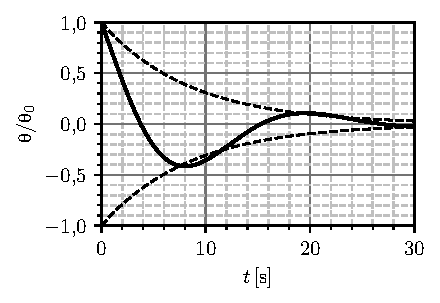
\includegraphics{fig/teleskop_plot.pdf}
    \caption{Временски дијаграм сиганала $\upepsilon(t)$.}
    \label{fig:\ID.res}
\end{figure}

(д) Тражени разултат може се показати скраћеним поступком. У случају када је комета са неким убрзањем, у том случају постоји и члан облика 
$\upalpha t^2$ у изразу за тренутни положај, односно Лапласова трансформација тог сигнала 
биће у облику $\Uptheta(s) = \dfrac{\cdot}{s^3}$ па онда уместо потирања чланова 
у изразу \ref{ID.eq1}, преостаје један пол у нули, односно $E(s) \sim \dfrac{\cdot}{s}$.
Па се онда применом теореме о коначној вредности добија 
$\upepsilon(\infty) = \lim_{s \to 0} s E(s) \sim \lim_{s \to 0} \cancel{s} \dfrac{\cdot}{\cancel{s}}$, па је 
добијени израз у општем случају различит од нуле. Заинтересованом читаоцу препоручујемо да овај поступак спроведе и 
формално, том приликом, налази се вредност $\upepsilon(\infty)$ која представља констатну грешку разматраног система. 
